\documentclass[tikz]{standalone}

\usepackage{amsmath}
\usepackage{amssymb}

\begin{document}

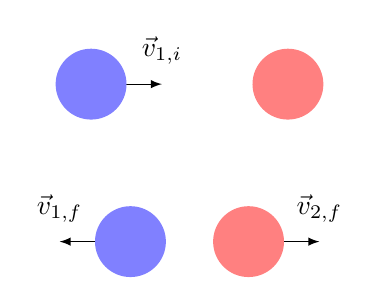
\begin{tikzpicture}
    \draw[-latex] (0.4-0.5,0)--(0.9-0.5,0) node [label=above:{$\Vec{v}_{1,i}$}] {};
    \fill[blue!50] (-0.5,0) circle (0.45);
    \node (a) at (0,-2){};
    \draw[-latex] (a) -- ++(180:0.9) node [label=above:{$\Vec{v}_{1,f}$}] {};
    \fill[blue!50] (a) circle (0.45);
    \node (b) at (1.5,-2){};
    \draw[-latex] (b) -- ++(0:0.9) node [label=above:{$\Vec{v}_{2,f}$}] {};
    \fill[red!50] (2,0) circle (0.45);
    \fill[red!50] (b) circle (0.45);
    \end{tikzpicture}

\end{document}